\section{From Particles to Fields}
In this lecture, we will look at a chain of atoms, and a chain of ferromagnetic spins.

\subsection{Phonons}

We consider atoms of mass $m$ connected by springs of spring constant $k_s$, with equilibrium $a$. We can notate the displacement of the $n$th atom from its equilibrium position as $\phi_n$, and $x_n$ the distance of the $n$th atom from the end of the string. 

\begin{figure}[htbp]
    \centering
    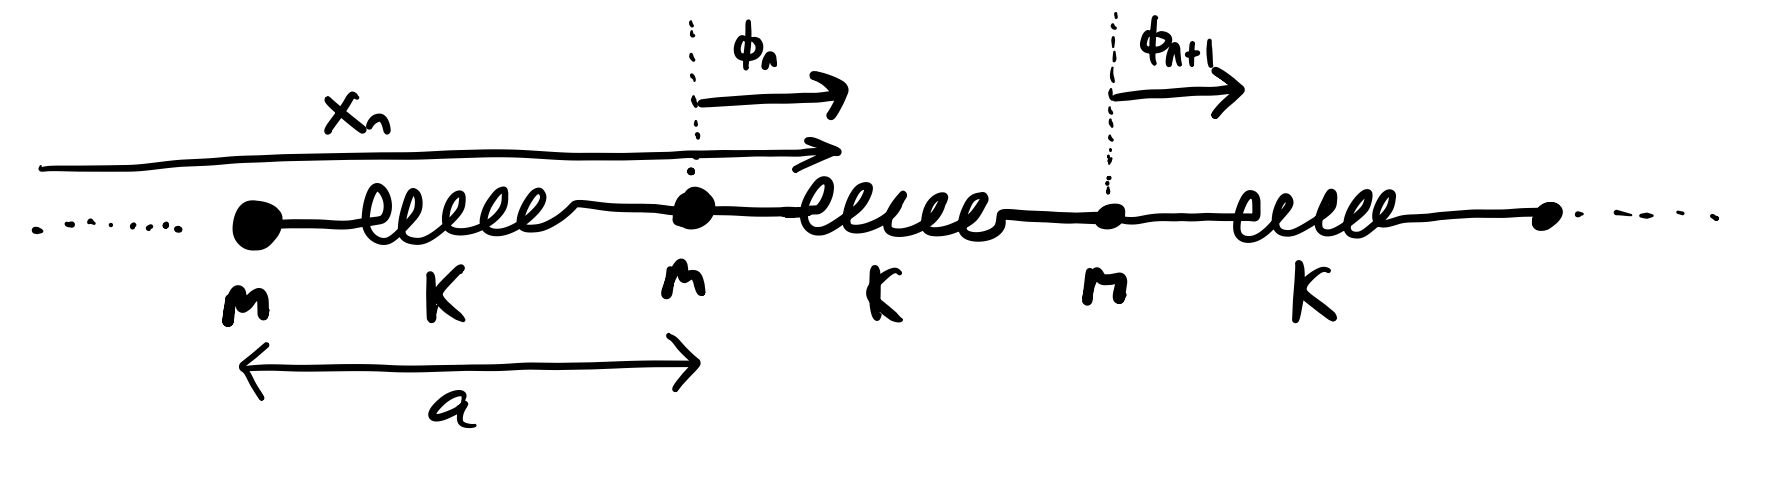
\includegraphics[scale=0.4]{Lectures/Figures/Atom_spring_chain.png}
    \caption{Diagram of a chain of atoms connected by springs.}
    \label{fig:Atom_spring_chain}
\end{figure}

The Lagrangian of the system is then:
\begin{equation}
    L = T - V = \sum_{i=1}^N \left[\frac{1}{2}m\dot{x}_n^2 - \frac{k_s}{2}\left(x_{n+1} - x_n - a\right)^2\right] = \sum_{n=1}^N \left[\frac{1}{2}m\dot{\phi}_n^2 - \frac{k_s}{2}\left(\phi_{n+1}-\phi_n\right)^2\right]
\end{equation}
notice there is a potential energy piece and a kinetic energy piece, both quadratic. We will want to solve for the eigenmodes of these problem. There are $N$ degrees of freedom and as such we expect to find $N$ eigenmodes.

This problem is solvable! We can write down the equation of motion of the springs; this is just nearest neighbour couplings so we can write down an analytic solution.

We promote:
\begin{equation}
    \phi_n \to a^{1/2}\phi(x)
\end{equation}
with the $a^{1/2}$ introduced for dimensional purposes, namely in such a way that we measure position in units of $\frac{x}{a}$, i.e. making it dimensionless. Then:
\begin{equation}
    (\phi_{n+1} - \phi_n) \to a^{3/2}\p_x \phi(x)
\end{equation}
Finally, we convert from a discrete sum to an integral:
\begin{equation}
    \sum \to \frac{1}{a}\int_0^{L=N_a}dx
\end{equation}
Thus the Lagrangian becomes a \emph{functional} (i.e. a function of a function) of a field:
\begin{equation}
    L[\phi] = \int_0^x \mathcal{L}(\phi, \p_x\phi, \dot{\phi})
\end{equation}
where $\mathcal{L}$ is the Lagrangian density:
\begin{equation}
    \mathcal{L} = \frac{1}{2}m\dot{\phi}^2 - \frac{k_s a^2}{2}(\p_x \phi)^2.
\end{equation}
We then write down the classical action:
\begin{equation}
    S[\phi] = \int dt L[\phi]
\end{equation}
Currently the field $\phi$ is not determined; it is a function of $x, t$. Our next task is to look for solutions that minimize the action.

To this end, we have the Euler-Lagrange equation:
\begin{equation}
    \dpd{\LL}{\phi} - \dod{}{t}\dpd{\LL}{\dot{\phi}} - \dod{}{x}\dpd{L}{(\p_x \phi)} = 0
\end{equation}
which is derived from the principle of least action. Working out the Euler Lagrange equation, we get the expected result:
\begin{equation}
    \boxed{[m\p_t^2 - (k_s a^2)\p_x^2]\phi(x, t) = 0}
\end{equation}
this is a wave equation! What we can see is it describes sound waves. Notice that the above equation is translation invariant, and as such the general solution is the sum of a right and left handed wave:
\begin{equation}
    \phi_+(x + vt) - \phi_-(x - vt)
\end{equation}
with velocity:
\begin{equation}
    v = a\sqrt{\frac{k_s}{m}}.
\end{equation}

Often however, it is common to look at this equation and say that it is simplest to study it in terms of Fourier modes; consider solutions:
\begin{equation}
    \phi(x, t) = \phi_0e^{i(\omega t - kx)}
\end{equation}
which plugging into the wave equation gives us the dispersion relation:
\begin{equation}
    \omega = vk
\end{equation}
The waves oscillate in time and in space.

Going back to the discrete case, we have the eigenmodes:
\begin{equation}
    \phi_n(t) = \sum_{k}\frac{1}{\sqrt{N}}e^{i(\omega_k t - k n a)}
\end{equation}
with dispersion:
\begin{equation}
    \omega(k) = 2\sqrt{\frac{k_s}{m}}\abs{\sin(\frac{k a}{2})}
\end{equation}
This solution knows about the discreteness of the lattice. Going to the continuum, we lost something, but we have a much simpler theory. In particular, the theory is good for small $k$/large wavelengths. The coarse graining made us lose information about the short-wavelength modes; we should not use the field theory for microscopic wavelengths. But, say for populating the chain with low-$T$ bosons (i.e. low energy bosons) this captures the phenomenology well. 

The dispersion curves looks like:
\begin{figure}[htbp]
    \centering
    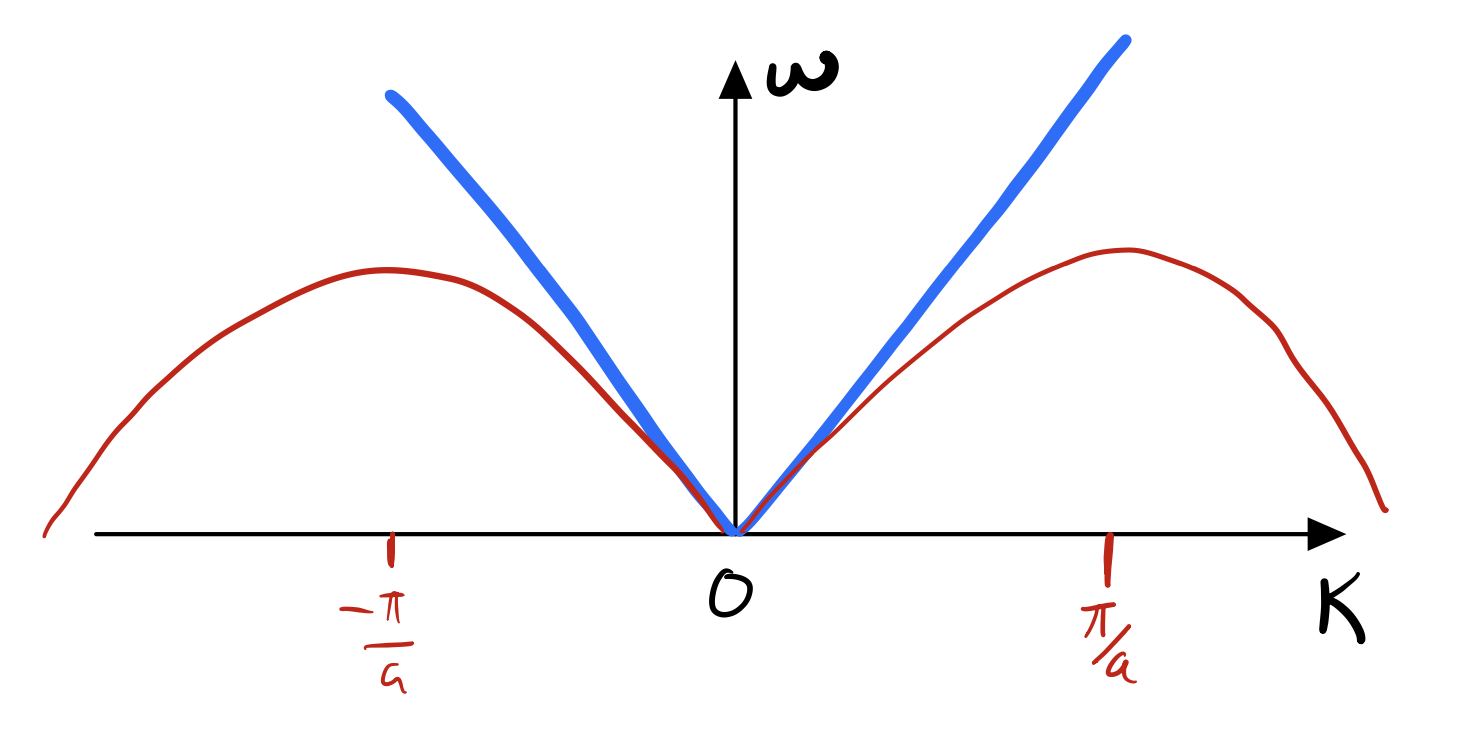
\includegraphics[scale=0.4]{Lectures/Figures/Phonon_dispersion.png}
    \caption{Continuum and Discrete Dispersion. The continuum dispersion is linear in $k$, while the discrete dispersion is $\sim \abs{\sin(k)}$. The two dispersion relations agree for small $k$/large wavelengths/small energies.}
    \label{fig:Phonon_dispersion}
\end{figure}

We can now use this to do thermodynamics! We can write down the internal energy:
\begin{equation}
    E(T) = E_0 + \sum_k \hbar \omega(k)\left[\avg{n_k} + \frac{1}{2}\right]
\end{equation}
where:
\begin{equation}
    \avg{n_k} = \frac{1}{e^{\frac{\hbar\omega}{k_BT}} - 1}
\end{equation}
In the limit where $k_B T \ll \hbar\omega$, $\hbar\omega(k) \to \hbar v k$ and the energy goes as $\sim T^2$. This is the well known thermodynamic dependence of the spring chain.

\subsection{Ferromagnetic Heisenberg Chain}
We consider the quantum Hamiltonian:
\begin{equation}
    \hat{H} = -J\sum_{m=1}^{N-1} \hat{\v{S}}_m \cdot \hat{\v{S}}_{m+1}
\end{equation}
where we take the coupling $J > 0$ such that the spins aligning result in lowered energy (i.e. we are describing a ferromagnet). At each site we have spin operators:
\begin{equation}
    [\hat{S}^i_m, \hat{S}^j_n] = i\delta_{mn}\e^{ijk}\hat{S}^k_n
\end{equation}
with $\delta_{mn}$ the Kronecker delta (which tells us that the spin operators only have nontrivial commutation on the same site) and $\e^{ijk}$ is the totally anti-symmetric tensor. We denote the total spin as $S$, a number (can be 1/2, 1, 3/2, etc.). We can consider the eigenstates of $\hat{S}^z$:
\begin{equation}
    \hat{S}^z_m\ket{s_m} = s\ket{s_m}.
\end{equation}
where $\ket{S_m}$ form a ladder of states from $s = -S, -S+1, \ldots, S-1, S$. We guess the ground state:
\begin{equation}
    \ket{\Omega} = \bigotimes_{m=1}^N \ket{S_m}
\end{equation}
i.e. all the spins are spin up. This clearly minimizes the energy, as for each coupling term $\v{S}_m \cdot \v{S}_{m+1}$ we get energy $-JS$ and so the total energy of $\ket{\Omega}$ is $-JSN$. Note however in writing this ground state down we broke some symmetry, as indeed the spins could be all aligned in any direction, and we would get the same ground state energy.

Recall that on a single site, we can have the raising/lowering operators:
\begin{equation}
    \hat{S}^\pm_m = \hat{S}^x_m \pm i \hat{S}^y_m
\end{equation}
which takes us up/down the ladder of $\ket{s_m}$ eigenstates. We can now rewrite our Hamiltonian to be of the form:
\begin{equation}
    \hat{H} = -J\sum_m \left(\hat{S}^z_m\hat{S}^z_{m+1} + \frac{1}{2}\left(\hat{S}^+_m\hat{S}^-_{m+1} + \hat{S}^-_m\hat{S}^+_{m+1}\right)\right)
\end{equation}

We now play a trick, namely the Holstein-Primakoff transformation. We define new operators (sometime known as magnon variables):
\begin{equation}
    \hat{S}^z_m = S - \hat{a}^\dag_m \hat{a}_m
\end{equation}
\begin{equation}
    \hat{S}^+_m = \left(2S - \hat{a}^\dag_m \hat{a}_m\right)^{1/2}a
\end{equation}
\begin{equation}
    \hat{S}^-_m = \hat{a}^\dag_m \left(2S - \hat{a}^\dag_m \hat{a}_m\right)^{1/2}
\end{equation}
where:
\begin{equation}
    [\hat{a}_m, \hat{a}_n^\dag] = \delta_{mn}
\end{equation}
It can be verified that this transformation is \emph{exact} (though it looks strange!) as it preserves the spin commutation relations. Why does this work? Intuitively, we have introduced the bosons through the operators $\hat{a}, \hat{a}^\dag$; the ladder of spin states look like the ladder of spin states (just that one is an infinite, and one is a finite ladder). But the square roots actually make sure that the dimensionality of our Hilbert space is preserved, because when I hit the walls of $\pm S$, the state vanishes. However it is instructive to consider the case where $S$ is large:

Let us Taylor expand $\hat{S}^\pm$:
\begin{equation}
    \hat{S}^+_m \approx \sqrt{2S}\hat{a}_m + \frac{O(\hat{a}_m^\dag \hat{a}_m \hat{a}_m)}{\sqrt{2S}}
\end{equation}
if $S \to \infty$, then we can throw away all but the first order term. Interestingly, it has a habit of working even when $S = \frac{1}{2}$. Let us write the Hamiltonian to second order in the operators:
\begin{equation}
    \hat{H} = -JNS^2 + JS\sum_m\left[\hat{a}^\dag_m\hat{a}_m + \hat{a}^\dag_{m+1}\hat{a}_{m+1} - \hat{a}^\dag_m \hat{a}_{m+1} - \hat{a}^\dag_{m+1}\hat{a}_m\right] + O(S^0)
\end{equation}
The number operator terms come from the $\hat{S}^z$, while the exchange terms come from the $\hat{S}^\pm$ cross terms. As such, we have now rewrote the Hamiltonian in terms of bosonic modes. Because this is periodic, the natural thing to do is to go back to the phonon problem in the discrete sense. There, we went into momentum space, and we shall do that again here:
\begin{equation}
    \tilde{\hat{a}}_k = \frac{1}{\sqrt{N}}\sum_m e^{ikm}\hat{a}_m
\end{equation}
where the $\tilde{\hat{a}}_k$ corresponds to a momentum annihilation operator and $\hat{a}_m$ corresponds to a position annihilation operator. Note that the momentum operators obey the same algebra:
\begin{equation}
    [\tilde{\hat{a}}_k, \tilde{hat{a}}^\dag_{k'}] = \delta_{kk'}
\end{equation}
which transforms the Hamiltonian into:
\begin{equation}
    \hat{H} = -JNS^2 + \sum_k \omega_k \tilde{\hat{a}}^\dag_k \tilde{\hat{a}}_k
\end{equation}
where:
\begin{equation}
    \omega_k = 4J\sin^2(\frac{k}{2})
\end{equation}
This is a quadratic (at small $k$) dispersion relation. Note that we still have a zero mode at $k = 0$ where the symmetry is preserved. Note also that in the HW, you will solve the classical version of this problem, and find the same dispersion.

\begin{figure}[htbp]
    \centering
    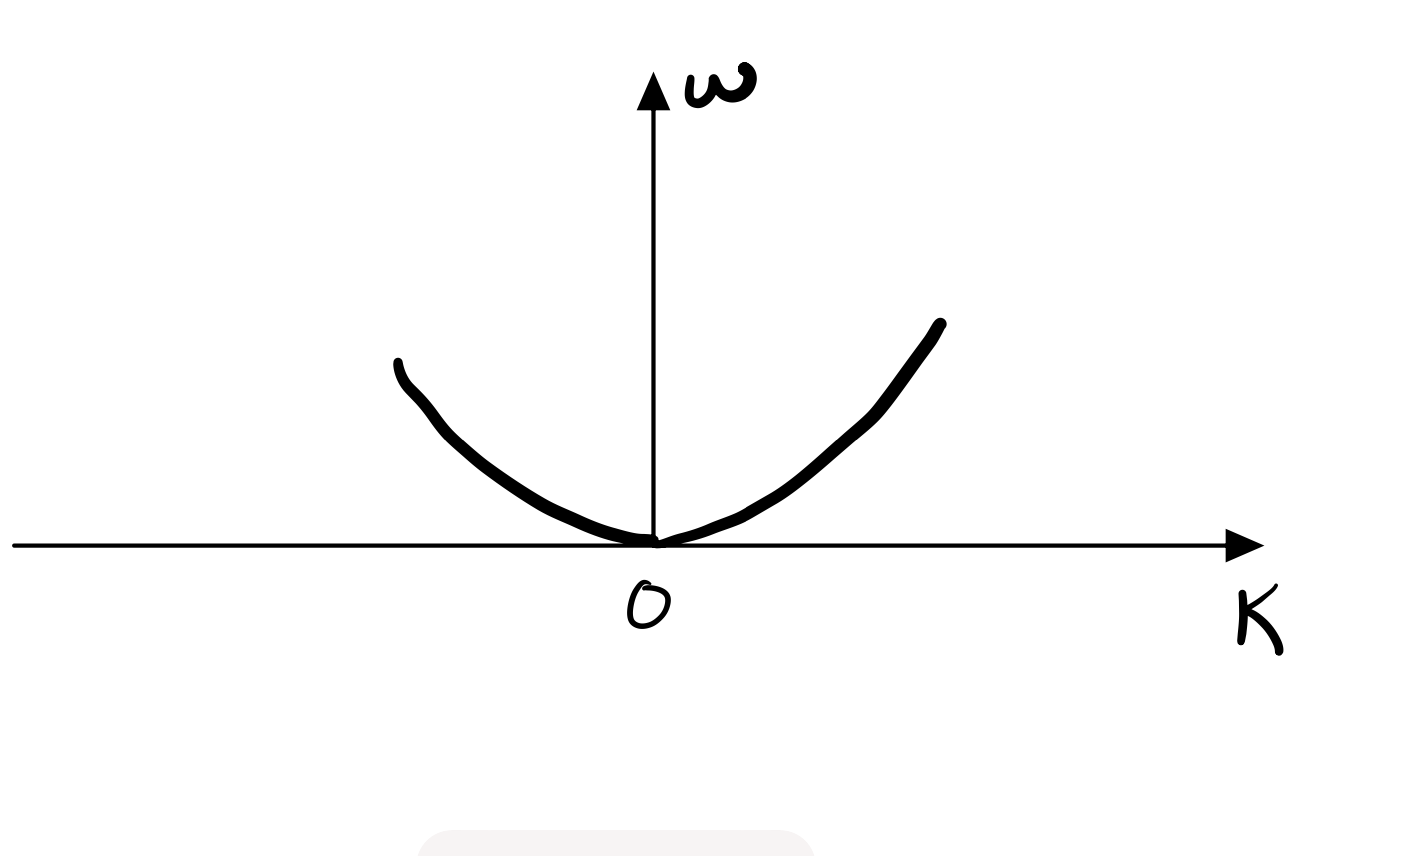
\includegraphics[scale=0.4]{Lectures/Figures/FM_spin_dispersion.png}
    \caption{Small $k$ dispersion relation for the ferromagnetic Heisenberg spin chain. For small $k$, the dispersion is quadratic.}
    \label{fig:FM_spin_dispersion}
\end{figure}

We call these objects ``spin waves''. This is clearly an approximation, as we have ignored the $O(S^0)$ terms in the Hamiltonian which include terms such as $\hat{a}^\dag a \hat{a}^\dag a$ which correspond to interactions between spin waves. So long as we stay near the zero mode, there is ``nowhere to go'' so the interactions can be neglected (if we look at large $k$ modes on the other hand, the interactions become relevant). 

A naive field theory for this would produce $\omega_k \sim k$, but it turns out spin conservation + rotational invariance gives us $\omega_k \sim k^2$. On Friday, we will look at the antiferromagnetic version of this problem, where we will see we obtain $\omega_k \sim k$ (due to vacuum fluctuations).
